\subsubsection{UC5 - Visualizzazione unità}
    \begin{figure}[h!]
        \centering
        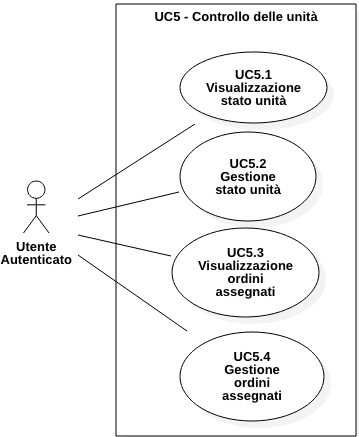
\includegraphics[width=9cm]{images/uc5.png}  
        \caption{Diagramma UC5 - Visualizzazione unità}
    \end{figure}
    \begin{itemize}
        \item \textbf{Attori primari:} utente autenticato;
        \item \textbf{Descrizione:} l'utente intende visualizzare in dettaglio ed in tempo reale le proprietà di un'unità;
        \item \textbf{Scenario principale:} l'utente visualizza:
        \begin{itemize}
            \item le caratteristiche dell'unità (UC5.1);
            \item la coda degli ordini assegnati all'unità (UC5.2).
        \end{itemize}
        \item \textbf{Precondizione:} l'utente accede all'ambiente dedicato alle proprietà dell'unità;
        \item \textbf{Postcondizione:} l'utente visualizza in tempo reale le proprietà dell'unità.
    \end{itemize}

        \subsubsection{UC5.1 - Visualizzazione caratteristiche unità}
        \begin{itemize}
            \item \textbf{Attori primari:} utente autenticato;
            \item \textbf{Descrizione:} l'utente intende visualizzare le seguenti caratteristiche dell'unità:
            \begin{itemize}
                \item codice identificativo univoco;
                \item coordinate della posizione attuale all'interno della mappa;
                \item stato dell'unità che può essere:
                \begin{itemize}
                    \item \underline{Going to X}: dove X è il codice identificativo univoco del \glock{POI} (punto di consegna o base di ricarica) verso cui l'unità si sta dirigendo;
                    \item \underline{Stop}: l'unità, pur rimanendo accesa e connessa, rimane ferma nella sua posizione attuale;
                    \item \underline{Base}: come \underline{Stop} ma l'unità si trova nella base di ricarica pronta per ricevere nuovi ordini;
                    \item \underline{Error Y}: come \underline{Stop} ma l'unità si trova ferma a causa di un errore con codice identificativo univoco Y; alcuni errori potrebbero essere irreversibili e richiedere un intervento fisico sull'unità;
                    \item \underline{Disconnected}: il sistema non rileva l'unità che potrebbe essere spenta o disconnessa per motivazioni impreviste;
                \end{itemize}
                \item velocità attuale;
                \item direzione (suggerita dal sistema) del prossimo passo.
            \end{itemize}
            \item \textbf{Scenario principale:} l'utente prende visione dello stato dell'unità;
            \item \textbf{Precondizione:} l'utente accede all'ambiente dedicato alle proprietà dell'unità;
            \item \textbf{Postcondizione:} l'utente visualizza in tempo reale le caratteristiche dell'unità.
        \end{itemize}

        \subsubsection{UC5.2 - Visualizzazione ordini assegnati}
        \begin{itemize}
            \item \textbf{Attori primari:} utente autenticato;
            \item \textbf{Descrizione:} l'utente intende visualizzare la coda degli ordini assegnati;
            \item \textbf{Scenario principale:} l'utente visualizza la coda degli ordini assegnati ovvero la lista dei \glock{POI} a cui effettuare la consegna prima di tornare alla base;
            \item \textbf{Precondizione:} l'utente accede all'ambiente dedicato alle proprietà dell'unità;
            \item \textbf{Postcondizione:} l'utente visualizza in tempo reale gli ordini assegnati all'unità.
        \end{itemize}


    \subsubsection{UC6 - Gestione unità}
    \begin{figure}[h!]
        \centering
        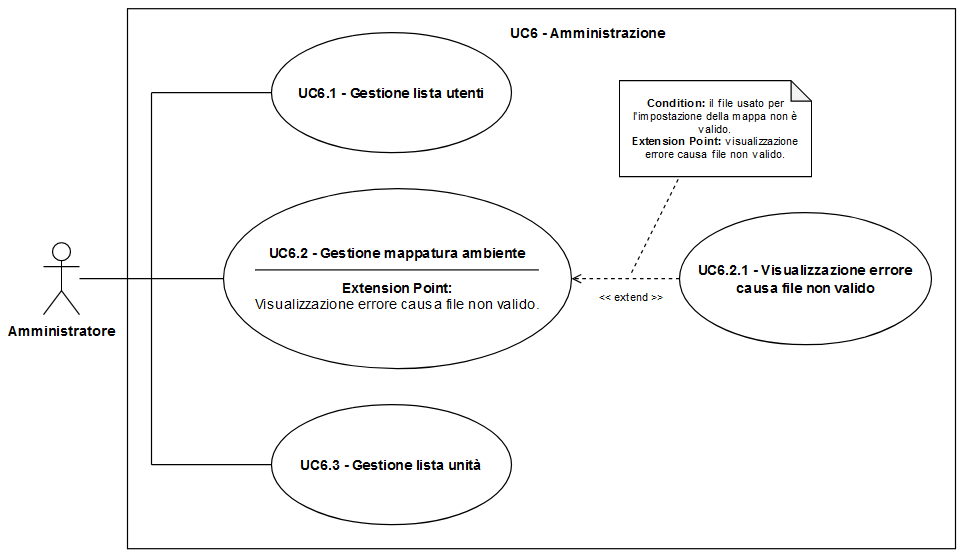
\includegraphics[width=10cm]{images/uc6.png}
        \caption{Diagramma UC6 - Gestione unità}
    \end{figure}
    \begin{itemize}
        \item \textbf{Attori primari:} utente autenticato;
        \item \textbf{Descrizione:} l'utente intende assegnare ordini all'unità o cambiarne lo stato;
        \item \textbf{Scenario principale:} l'utente impartisce determinati comandi per modificare lo stato dell'unità:
        \begin{itemize}
            \item Start (UC6.1);
            \item Stop (UC6.2);
            \item Go Back (UC6.3);
            \item Shutdown (UC6.4).
        \end{itemize}
        l'utente, inoltre, assegna (UC6.5) o elimina (UC6.6) ordini dalla coda degli ordini dell'unità;
        \item \textbf{Precondizione:} l'utente accede all'ambiente dedicato alla gestione dell'unità;
        \item \textbf{Postcondizione:} l'utente modifica in tempo reale lo stato dell'unità e la coda degli ordini.
    \end{itemize}

        \subsubsection{UC6.1 - Comando start}
        \begin{itemize}
            \item \textbf{Attori primari:} utente autenticato;
            \item \textbf{Descrizione:} l'utente intende impostare lo stato dell'unità in modo che consegni tutti gli ordini assegnati per poi tornare alla base;
            \item \textbf{Scenario principale:} partendo da un'unità con stato \underline{Base} o \underline{Stop}, l'utente rende \underline{Going to X} il nuovo stato dell'unità;
            \item \textbf{Precondizione:} l'utente accede all'ambiente dedicato alla gestione dell'unità;
            \item \textbf{Postcondizione:} l'utente modifica in tempo reale lo stato dell'unità portandolo allo stato \underline{Going to X}.
        \end{itemize}

        \subsubsection{UC6.2 - Comando stop}
        \begin{itemize}
            \item \textbf{Attori primari:} utente autenticato;
            \item \textbf{Descrizione:} l'utente intende impostare lo stato dell'unità in modo che, pur rimanendo accesa e connessa, rimanga nella posizione attuale;
            \item \textbf{Scenario principale:} l'utente rende \underline{Stop} il nuovo stato dell'unità;
            \item \textbf{Precondizione:} l'utente accede all'ambiente dedicato alla gestione dell'unità;
            \item \textbf{Postcondizione:} l'utente modifica in tempo reale lo stato dell'unità portandolo allo stato \underline{Stop}.
        \end{itemize}

        \subsubsection{UC6.3 - Comando go back}
        \begin{itemize}
            \item \textbf{Attori primari:} utente autenticato;
            \item \textbf{Descrizione:} l'utente intende impostare lo stato dell'unità in modo che, indipendentemente dalla situazione attuale della coda degli ordini, ritorni alla base;
            \item \textbf{Scenario principale:} partendo da un'unità con stato \underline{Start} o \underline{Stop}, l'utente rende \underline{Going to B} il nuovo stato dell'unità, dove B è la base;
            \item \textbf{Precondizione:} l'utente accede all'ambiente dedicato alla gestione dell'unità;
            \item \textbf{Postcondizione:} l'utente modifica in tempo reale lo stato dell'unità portandolo allo stato \underline{Going to B}.
        \end{itemize}

        \subsubsection{UC6.4 - Comando shutdown}
        \begin{itemize}
            \item \textbf{Attori primari:} utente autenticato;
            \item \textbf{Descrizione:} l'utente intende spegnere l'unità attualmente connessa, in modo immediato;
            \item \textbf{Scenario principale:} Ignorando stato attuale e qualsiasi ordine ancora assegnato, l'utente spegne l'unità in modo immediato portandola in stato \underline{Disconnected};
            \item \textbf{Precondizione:} l'utente accede all'ambiente dedicato alla gestione dell'unità;
            \item \textbf{Postcondizione:} l'utente modifica in tempo reale lo stato dell'unità portandolo allo stato \underline{Disconnected}.
        \end{itemize}

        \subsubsection{UC6.5 - Assegnazione nuovo ordine}
        \begin{itemize}
            \item \textbf{Attori primari:} utente autenticato;
            \item \textbf{Descrizione:} l'utente intende accodare un nuovo ordine;
            \item \textbf{Scenario principale:} l'utente assegna il nuovo ordine all'unità, ed inserisce l'identificativo del \glock{POI} da visitare per effettuare la consegna;
            \item \textbf{Precondizione:} l'utente accede all'ambiente dedicato alla gestione dell'unità;
            \item \textbf{Postcondizione:} l'utente modifica in tempo reale la coda degli ordini aggiungendo un nuovo ordine.
        \end{itemize}

        \subsubsection{UC6.6 - Eliminazione ordine assegnato}
        \begin{itemize}
            \item \textbf{Attori primari:} utente autenticato;
            \item \textbf{Descrizione:} l'utente intende eliminare un ordine in coda ad un'unità che si trova alla base;
            \item \textbf{Scenario principale:} l'utente elimina l'ordine dalla coda indipendentemente dalla sua posizione all'interno di essa;
            \item \textbf{Precondizione:} l'utente accede all'ambiente dedicato alla gestione dell'unità;
            \item \textbf{Postcondizione:} l'utente modifica in tempo reale la coda degli ordini eliminando un ordine.
        \end{itemize}
